\documentclass[10pt,aspectratio=43]{beamer}
\usetheme{CambridgeUS}
\usecolortheme{dolphin}
\usepackage{multimedia}
\usepackage{xcolor}
\usepackage{graphicx}
\usepackage[normalem]{ulem}
\usepackage{amsmath}
\usepackage{tikz}
\usetikzlibrary{positioning, shapes.geometric, arrows.meta}
\usepackage{pgfplots}
\pgfplotsset{compat=1.17}
\graphicspath{{figures/lec/}}
\begin{document}
%--------------------------------------------------------------------------- SLIDE 1: Halting Problem & Problem Classification ----------------------------------------------------------------------------------------
\begin{frame}
  \frametitle{Halting Problem \& Problem Classification}
  
  \textbf{Halting Problem:}
  \begin{itemize}
      \item No general algorithm can solve it for all cases (undecidable)
      \vspace{3pt}
      \item Not solvable in any amount of time — not even non-polynomial
      \vspace{3pt}
      \item No formal proof method exists to solve it algorithmically
  \end{itemize}
  
  \vspace{0.5cm}
  
  \textbf{Classifying Problems:}
  \begin{itemize}
      \vspace{5pt}
      \item Examples of problems not known to be solvable in polynomial time:
      \begin{itemize}
          \item \textbf{Longest Path Problem}
          \vspace{3pt}
          \item \textbf{Travelling Salesman Problem (TSP)}
          \vspace{3pt}
          \item \textbf{Subset Sum Problem}
          \vspace{3pt}
          \item \textbf{Clique Problem}
          \vspace{3pt}
          \item \textbf{Independent Set Problem}
      \end{itemize}
  \end{itemize}
\end{frame}


%--------------------------------------------------------------------------- SLIDE X: Defining a Problem in Algorithms ----------------------------------------------------------------------------------------
\begin{frame}
  \frametitle{Defining a Problem in Algorithms}

  \textbf{What is a computational problem?}
  \begin{itemize}
      \item Given an input, compute an output that satisfies some condition.
      \item Often represented as a function: $x \rightarrow y$
  \end{itemize}

  \vspace{0.3cm}

  \textbf{General Case}
  \begin{itemize}
      \item \textbf{Input:} A list of numbers $x$
      \item \textbf{Output:} A corresponding list $y$, where each $y_i$ depends on $x_i$
      \item Mapping a complex output list can be messy and hard to analyze or optimize.
  \end{itemize}

  \vspace{0.3cm}

  \textbf{Simplifying with Decision Problems}
  \begin{itemize}
      \item To reduce complexity, we often ask a simpler question for each input:
            \begin{itemize}
                \item Is the answer \textbf{yes (1)} or \textbf{no (0)}?
            \end{itemize}
      \item These are called \textbf{decision problems}.
      \item Decision problems are easier to classify and analyze, especially in complexity theory.
  \end{itemize}
\end{frame}
%  \begin{frame}
%    \frametitle{Defining a Problem in Algorithms (Continued)}
%  \textbf{Solution example:}
%  \begin{itemize}
%      \item \textbf{Input:} A graph
%      \vspace{3pt}
%      \item \textbf{Task:} Find a Minimum Spanning Tree (MST)
%      \vspace{3pt}
%      \item \textbf{Output:} A tree connecting all vertices with minimal total edge weight
%  \end{itemize}
%\end{frame}

%--------------------------------------------------------------------------- SLIDE 5: MST - Decision Version ----------------------------------------------------------------------------------------
\begin{frame}
  \frametitle{MST – Decision Version}
  
  \textbf{Input:}
  \begin{itemize}
      \item A weighted graph $G$
      \vspace{3pt}
      \item A number $p$
  \end{itemize}
  
  \vspace{0.3cm}
  
  \textbf{Output:}
  \begin{itemize}
      \item \texttt{1} if there exists an MST in $G$ with total weight $\leq p$
      \vspace{3pt}
      \item \texttt{0} otherwise
  \end{itemize}
  
  \vspace{0.5cm}
  
  \textbf{Simplified Form:}
  \begin{itemize}
      \item $G, p \rightarrow \texttt{1}$ \quad if $\exists$ an MST in $G$ with weight $\leq p$
      \vspace{3pt}
      \item Output is binary: \texttt{1} or \texttt{0}
  \end{itemize}
  
  \vspace{0.3cm}
    \end{frame}
    
%  \begin{frame}
%    \frametitle{MST – Decision Version (Continued)}
%  \begin{block}{Key Characteristics}
%      \begin{itemize}
%          \item Converts optimization problem to decision problem
%          \vspace{3pt}
%          \item Binary output simplifies analysis
%          \vspace{3pt}
%          \item Maintains core computational challenge
%      \end{itemize}
%  \end{block}
%\end{frame}


%--------------------------------------------------------------------------- SLIDE 6: Optimisation Problem - MST ----------------------------------------------------------------------------------------
\begin{frame}
  \frametitle{Optimisation Problem – MST}
  
  \textbf{Type:}
  \begin{itemize}
      \item Optimisation Problem (minimization)
  \end{itemize}
  
  \vspace{0.3cm}
  
  \textbf{Original Formulation:}
  \begin{itemize}
      \item \textbf{Input:} A weighted graph $G$
      \vspace{3pt}
      \item \textbf{Output:} The minimum total weight of its MST
  \end{itemize}
  
  \vspace{0.3cm}
  
  \textbf{Goal:}
  \begin{itemize}
      \item Find the value (not just existence) of the minimum spanning tree
      \vspace{3pt}
      \item Maps input to a numeric output, not just 0/1
  \end{itemize}
\end{frame}

%--------------------------------------------------------------------------- SLIDE 7: Decision vs. Optimisation ----------------------------------------------------------------------------------------
\begin{frame}
  \frametitle{Decision vs. Optimisation}

  \begin{columns}
    % Left column: Text
    \begin{column}{0.6\textwidth}
      \textbf{Question 1:}
      \begin{itemize}
          \item If the decision version is solved in $O(n^2)$, 
                can we solve the optimisation version in $O(n \log n)$?
          \item Approach: binary search over possible values of $p$
      \end{itemize}

      \vspace{0.4cm}
      \textbf{Question 2:}
      \begin{itemize}
          \item Can we solve the decision problem using the optimisation problem?
          \item Yes:
            \begin{itemize}
                \item Compute MST weight using optimisation
                \item Compare result to $p$: Output 1 if $\leq p$, else 0
                \item Simple post-check after solving optimisation
            \end{itemize}
      \end{itemize}
    \end{column}

    % Right column: Image
    \begin{column}{0.4\textwidth}
      \begin{figure}
        \centering
        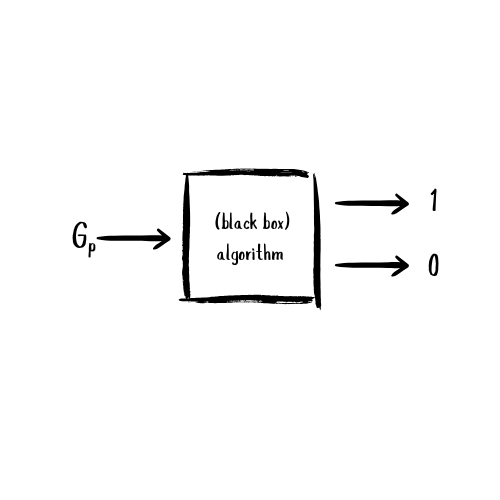
\includegraphics[width=\linewidth]{figures/lec/optmi.png}
      \end{figure}
    \end{column}
  \end{columns}
\end{frame}
%--------------------------------------------------------------------------- SLIDE 8,9: Understanding NP ----------------------------------------------------------------------------------------
\begin{frame}
  \frametitle{Understanding NP}
  
  \textbf{NP (Nondeterministic Polynomial time):}
  \begin{itemize}
      \item Class of problems for which yes instance can be verified
  \end{itemize}
  
  \vspace{0.3cm}
  
  \textbf{Key Concepts:}
  \begin{itemize}
      \item \textbf{Instance:} fixed problem input
      \vspace{0.2cm}
      \item \textbf{Prover–Verifier Model:}
      \begin{itemize}
          \item \textbf{Prover:} Provides a proposed solution (0 or 1)
          \item If the answer is ``No'' $\rightarrow$ no requirement to prove
          \item If the answer is ``Yes'' $\rightarrow$ must provide polynomial-time verifiable certificate
      \end{itemize}
  \end{itemize}
\end{frame}

\begin{frame}
  \frametitle{Examples of NP Problems}
  
  \textbf{Subset Sum:}
  \begin{itemize}
      \item Given a set of integers, is there a subset whose sum is zero?
      \vspace{3pt}
      \item If yes, the subset itself serves as a certificate verifiable in polynomial time
  \end{itemize}
  
  \vspace{0.5cm}
  
  \textbf{Longest Path:}
  \begin{itemize}
      \item Given a graph and integer $k$, is there a simple path of length $\geq k$?
      \vspace{3pt}
      \item If yes, the specific path can be checked efficiently
  \end{itemize}
  
  \vspace{0.5cm}
  
  \begin{block}{NP Characteristics}
      \begin{itemize}
          \item Focuses on \textbf{verification} rather than solution
          \vspace{3pt}
          \item The certificate must be \textbf{polynomial} in size
          \vspace{3pt}
          \item Verification must run in \textbf{polynomial time}
      \end{itemize}
  \end{block}
\end{frame}


\begin{frame}
  \frametitle{An open question}

  \begin{minipage}{0.48\textwidth}
    \centering
    Is the picture like this?

    \vspace{0.3cm}

    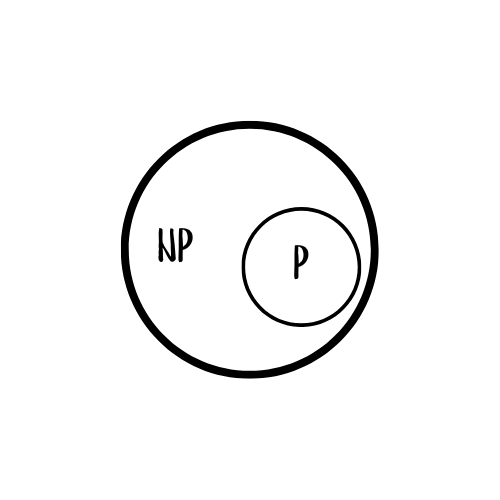
\includegraphics[width=\linewidth]{figures/lec/np1.png} 
  \end{minipage}
  \hfill
  \begin{minipage}{0.48\textwidth}
    \centering
    Or like this?

    \vspace{0.3cm}

    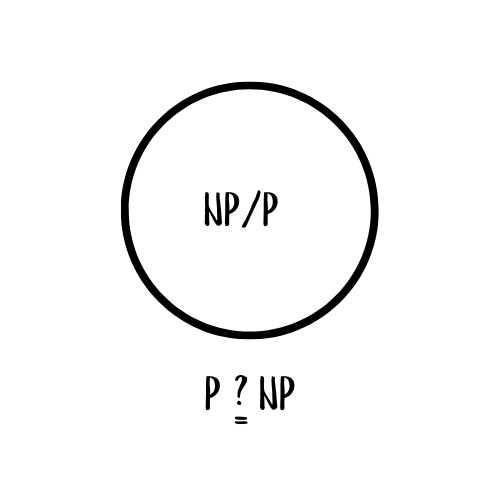
\includegraphics[width=\linewidth]{figures/lec/np2.png} 
  \end{minipage}
\end{frame}

%--------------------------------------------------------------------------- SLIDE 11: Complexity Classes ----------------------------------------------------------------------------------------
\begin{frame}
  \frametitle{Complexity Classes}


  \begin{block}{Reduction: $P_1$, $P_2$ (2 problems)}
    \begin{itemize}
        \item Is a way to transform $P_1$ instance ($X$) to $P_2$ instance ($Y$) such that:
             If $P_1(X)$ is a yes-instance, then $P_2(Y)$ must also be a yes-instance and the other way around
        \item Basically solve $P_1$ using $P_2$
    \end{itemize}
  \end{block}
  
        \vspace{0.3cm}
  \textbf{NP-hard:}
  \begin{itemize}
      \item Is a class of problems $y$ such that every $x$ in NP can be poly-reduced to [some] $y$
  \end{itemize}
      \vspace{0.3cm}
  \textbf{NP-complete:}
  \begin{itemize}
      \item Problems which are in NP $\cap$ NP-hard
  \end{itemize}
\end{frame}


% -----Slides 12 
\begin{frame}
    \frametitle{Longest Path Problem}
    \begin{itemize}
        \item The \textbf{Longest Path} problem is an \textbf{NP-Hard} problem.
        \item It involves finding the longest simple path between two nodes in a graph.
        \item Finding the longest path cannot be done efficiently in polynomial time.
        \item \textbf{NP-Hard} means the problem is at least as hard as any problem in NP.
    \end{itemize}
\end{frame}
%% ----Slide 13
%\begin{frame}
%    \frametitle{What is Reduction?}
%
%    \begin{block}{Definition}
%        \textbf{Reduction} is the process of transforming one problem into another problem, such that a solution to the new problem can be used to solve the original problem.
%    \end{block}
%
%    \vspace{0.5em}
%
%    \begin{itemize}
%        \item \textbf{Goal:} To show that solving one problem is at least as hard as solving another.
%        \item A reduction from problem \textbf{A} to problem \textbf{B} means:
%        \begin{itemize}
%            \item We can transform an instance of problem \textbf{A} into an instance of problem \textbf{B}.
%            \item Solving problem \textbf{B} gives us a solution to problem \textbf{A}.
%        \end{itemize}
%        \item \textbf{Polynomial-Time Reduction:} The transformation from \textbf{A} to \textbf{B} must be done in polynomial time.
%    \end{itemize}
%
%    \vspace{0.5em}
%
%    \begin{block}{Why is Reduction Important?}
%        Reductions allow us to prove that certain problems are \textbf{NP-Hard} by showing that a known NP-Hard problem can be reduced to the problem in question.
%    \end{block}
%\end{frame}

% ----Slide 14

\begin{frame}
    \frametitle{Relationship: NP $\Rightarrow$ Longest Path (via Reduction)}

    \begin{block}{What Does This Mean?}
        Every problem in \textbf{NP} can be \textbf{reduced} in polynomial time to the \textbf{Longest Path} problem.
    \end{block}

    \vspace{0.5em}

    \begin{itemize}
        \item This implies that \textbf{Longest Path} is \textbf{NP-Hard}.
        \item If we can solve the Longest Path problem, we can solve any problem in NP by reducing it to Longest Path.
        \item A \textbf{black-box solver} for Longest Path would allow us to solve all NP problems.
    \end{itemize}
\end{frame}

% ----Slide 15

\begin{frame}
    \frametitle{Why Are These Problems Important?}
    \begin{itemize}
        \item We cannot solve the Longest Path problem efficiently, but we can use it as a benchmark.
        \item The Longest Path problem is NP-Hard, meaning it is at least as hard as any other NP problem.
        \item This provides \textbf{evidence} that certain problems are fundamentally hard to solve.
    \end{itemize}

    \vspace{0.5em}

    \begin{block}{Significance}
        The difficulty of the Longest Path problem helps us understand the boundaries of \textbf{NP-completeness} and \textbf{NP-hardness}.
        This insight allows us to better grasp the complexity of other problems in \textbf{NP}.
    \end{block}
\end{frame}

% ----Slide 16

\begin{frame}
    \frametitle{Relationship: NP $\Rightarrow$ Longest Path (via Reduction)}

    \begin{block}{Key Insight}
        \textbf{Longest Path} is at the heart of \textbf{NP-Hard} problems. 
        If we could solve it efficiently in polynomial time, we would have a solution for all NP problems.
    \end{block}

    \vspace{0.5em}

    \begin{itemize}
        \item Solving Longest Path would imply \textbf{P = NP}, a famous unsolved question in computational complexity theory.
        \item The power of \textbf{polynomial-time reduction} means we can reduce any NP problem to Longest Path.
        \item This reduction shows that finding an efficient algorithm for Longest Path would unlock the ability to solve all NP problems.
    \end{itemize}
\end{frame}

% ----Slide 17

\begin{frame}
    \frametitle{The Challenge of Classifying Problems}

    \begin{block}{Why Classification Was Difficult}
        \begin{itemize}
            \item Early on, there was no clear way to compare the difficulty of problems.
            \item Researchers needed a way to formalize when one problem is "at least as hard" as another.
            \item This led to the idea of using \textbf{reductions} — transforming one problem into another.
        \end{itemize}
    \end{block}

    \vspace{0.5em}

    \begin{block}{The Breakthrough: Cook and Levin}
        \begin{itemize}
            \item In 1971, \textbf{Stephen Cook} introduced the concept of NP-Completeness with his proof that \textbf{SAT} is NP-Complete.
            \item Around the same time, \textbf{Leonid Levin} independently discovered similar ideas in the Soviet Union.
            \item Their work created the foundation for classifying many hard problems using reductions.
        \end{itemize}
    \end{block}

    \vspace{0.5em}
\end{frame}
\begin{frame}
    \frametitle{The Challenge of Classifying Problems (Continued)}
    \begin{block}{Impact}
        Cook and Levin's work made it possible to group problems by difficulty using reductions.
        This helped define what we now call \textbf{NP-Complete} problems — the hardest problems in NP.
    \end{block}
\end{frame}

% ----Slide 18
\begin{frame}
    \frametitle{Levin-Cook Theorem: Breakthrough and Impact}

    \begin{block}{The Breakthrough}
        \begin{itemize}
            \item \textbf{Stephen Cook (1971)} and \textbf{Leonid Levin (1973)} independently proved:
            \item The \textbf{Boolean Satisfiability Problem (SAT)} is the \textbf{first NP-Complete} problem.
        \end{itemize}
    \end{block}

    \vspace{0.5em}

    \begin{block}{Why It Mattered}
        \begin{itemize}
            \item SAT was the \textbf{first} known NP-Complete problem.
            \item Their result created a \textbf{starting point} to classify other problems.
            \item Any new problem could now be shown NP-Complete by \textbf{reducing SAT} to it.
            \item This was a \textbf{turning point} in computational complexity theory.
        \end{itemize}
    \end{block}
\end{frame}

%-----Slide 19
\begin{frame}
    \frametitle{SAT – The First NP-Complete Problem}

    \begin{block}{What is SAT?}
        \begin{itemize}
            \item \textbf{Input:} A Boolean formula in \textbf{Conjunctive Normal Form (CNF)}:
            \begin{itemize}
                \item CNF = AND of \textbf{clauses}, each clause is an OR of literals (variables or their negations).
            \end{itemize}
            \item \textbf{Goal:} Does there exist a true/false assignment that makes the formula true?
        \end{itemize}
    \end{block}

    \vspace{0.5em}

    \begin{block}{Example}
        \[
        (x_1 \lor x_2 \lor \lnot x_3) \land (x_2 \lor x_3) \land (\lnot x_1) \land (x_1 \lor x_4)
        \]

        \begin{itemize}
            \item \textbf{Clauses:}
            \begin{itemize}
                \item Clause 1: $(x_1 \lor x_2 \lor \lnot x_3)$
                \item Clause 2: $(x_2 \lor x_3)$
                \item Clause 3: $(\lnot x_1)$
                \item Clause 4: $(x_1 \lor x_4)$
            \end{itemize}
        \end{itemize}
    \end{block}
\end{frame}

% ----Slide 20

\begin{frame}
    \frametitle{Evaluating SAT Examples}

    \begin{itemize}
        \item \textbf{Simple examples:}
        \begin{itemize}
            \item $(x_1) \land (x_2)$ → \textbf{Satisfiable}, e.g., $x_1 = \text{T},\ x_2 = \text{T}$
            \item $(\lnot x_1) \land (x_2)$ → \textbf{Satisfiable}, e.g., $x_1 = \text{F},\ x_2 = \text{T}$
            \item $(\lnot x_1) \land (x_1)$ → \textbf{Unsatisfiable} (contradiction)
        \end{itemize}

        \vspace{0.5em}

        \item \textbf{Larger example:}
        \begin{itemize}
            \item Formula: $(x_1 \lor x_2 \lor \lnot x_3) \land (x_2 \lor x_3) \land (\lnot x_1) \land (x_1 \lor x_4)$
            \item Try assignment: $x_1 = \text{F},\ x_2 = \text{T},\ x_3 = \text{F},\ x_4 = \text{T}$
            \item \textbf{Check:} 
            \begin{itemize}
                \item Clause 1: $(F \lor T \lor T) = T$
                \item Clause 2: $(T \lor F) = T$
                \item Clause 3: $(T) = T$
                \item Clause 4: $(F \lor T) = T$
            \end{itemize}
            \item \textbf{Result:} Satisfied (All Clauses are True)
        \end{itemize}
    \end{itemize}
\end{frame}


% ----Slide 21

\begin{frame}
    \frametitle{Is SAT in NP?}

    \begin{itemize}
        \item \textbf{Yes}, SAT $\in$ NP.
        \item A satisfying assignment (e.g., $x_1 = T, x_2 = F, \dots$) acts as a \textbf{certificate}.
        \item Given such an assignment, we can \textbf{verify} whether the formula is true in \textbf{polynomial time}.
        \item \textbf{To prove SAT is NP-Complete}, we must also show it is \textbf{NP-Hard}.
        \item Cook and Levin showed all problems in NP can be \textbf{reduced to SAT}.
        \item \textbf{Implication:} If one problem in a set of problems is NP-Complete, all other problems in that set are also NP-Complete, as they can be reduced to each other.
    \end{itemize}
\end{frame}



% ----Slide 22

\begin{frame}
    \frametitle{Independent Set $\leq_p$ SAT}

    \begin{itemize}
        \item \textbf{Independent Set Problem}:
        \begin{itemize}
            \item Given a graph $G = (V, E)$ and an integer $k$
            \item Does there exist a subset $W \subseteq V$, with $|W| \geq k$, such that:
            \item No two vertices in $W$ are connected by an edge, i.e., $\forall u,v \in W: (u,v) \notin E$
        \end{itemize}

        \item \textbf{Reduction:} Independent Set $\leq_p$ SAT
        \begin{itemize}
            \item This means we can \textbf{transform any instance} of Independent Set into a SAT instance in polynomial time.
            \item So, if we could solve SAT efficiently, we could solve Independent Set efficiently.
        \end{itemize}
    \end{itemize}
\end{frame}
% Slide 5 - Independent Set Permutations Step 1
\begin{frame}
  \frametitle{Independent Set Permutations (Examples)}
  
  \begin{columns}[c]
    \begin{column}{0.48\textwidth}
      \begin{figure}
        \centering
        
\includegraphics[width=0.85\linewidth]{figures/lec/i1.png}
        \caption {$\{1\}$}
      \end{figure}
    \end{column}
    \begin{column}{0.48\textwidth}
      \begin{figure}
        \centering
        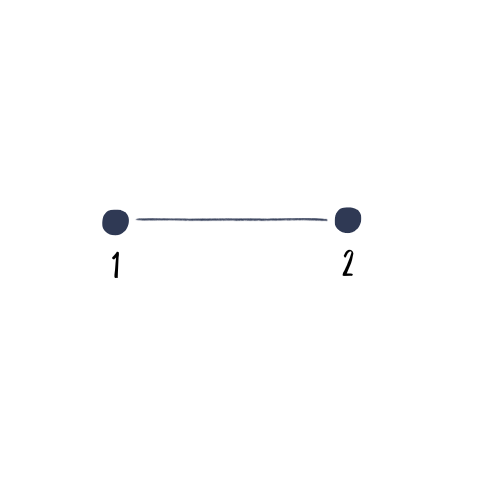
\includegraphics[width=0.85\linewidth]{figures/lec/i2.png}
        \caption {$\{1\}, \{2\}$}
      \end{figure}
    \end{column}
  \end{columns}
\end{frame}

% Slide 6 - Independent Set Permutations Step 2
\begin{frame}
  \frametitle{Independent Set Permutations (Examples)}
  
  \begin{figure}
    \centering
    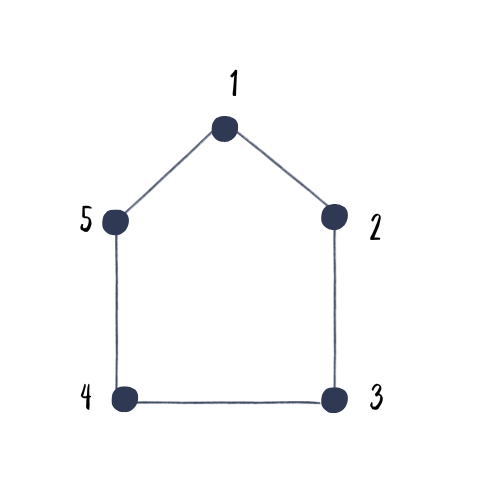
\includegraphics[width=0.4\linewidth]{figures/lec/i3.png}
    \caption {$\{1\}, \{2\}, \{3\}, \{4\}, \{5\}, \{5,3\}, \{2,4\}, \{1,3\}, \{1,4\}, \{5,2\}$}
  \end{figure}
\end{frame}
% ----Slide 23

\begin{frame}
    \frametitle{Maximum Independent Set (MIS)}
    \begin{itemize}
        \item \textbf{MIS Problem:} Given a graph $G = (V, E)$ and a number $k$
        \item Question: Is there an independent set of size $\geq k$ in $G$?
        \item MIS is \textbf{NP-Complete}.
        \item \textbf{Implication:} If you could solve MIS efficiently, you could solve SAT as well.
 \begin{figure}
    \centering
    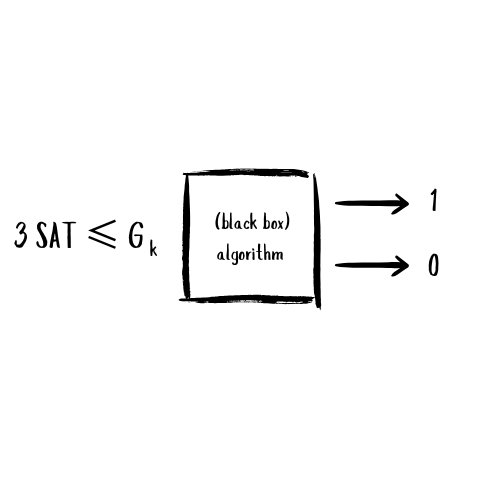
\includegraphics[width=0.4\linewidth]{figures/lec/MIS.png}
  \end{figure}
    \end{itemize}
\end{frame}

\begin{frame}
  \frametitle{Reduction: 3-SAT to Maximum Independent Set}
  
  \begin{block}{Example 3-SAT Formula}
    \begin{itemize}
      \item Variables: $x_1, x_2, x_3, x_4$
      \item Literals: $x_1, x_2, \lnot x_3, \lnot x_4$, etc.
    
    \end{itemize}
  \end{block}
  
  \vspace{0.3cm}
  
  \textbf{Reduction Process:}
  \begin{enumerate}
    \item Create a vertex for each literal in each clause
    \item Connect contradicting literals across clauses ($x_i$ and $\lnot x_i$)
    \item Connect literals from the same clause (making clause triangles)
    \item Set $k =$ number of clauses (here, $k = 4$)
  \end{enumerate}
  
   \begin{block}{Solve: }
      \[
      (x_1 \lor x_2 \lor \lnot x_3) \land
      (x_4 \lor x_2 \lor x_1) \land
      (\lnot x_4 \lor x_2 \lor x_3) \land
      (\lnot x_2 \lor x_1 \lor \lnot x_3)
      \]
  \end{block}
 
\end{frame}
% Slide 1_____________________________________________________________________
\begin{frame}
  \frametitle{Step 1}

 For each literal in your formula, create a vertex

  \begin{figure}[h!]
    \centering
    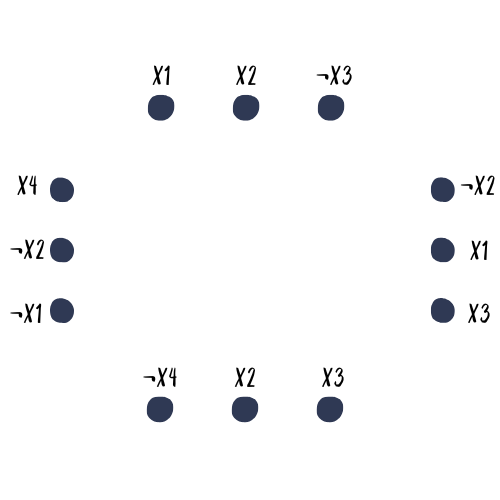
\includegraphics[width=0.45\linewidth]{figures/lec/reduction_1.png}
  \end{figure}
\end{frame}

% Slide 2
\begin{frame}
  \frametitle{ Step 2}

Across clauses, add an edge between each literal and its negation

  \begin{figure}[h!]
    \centering
    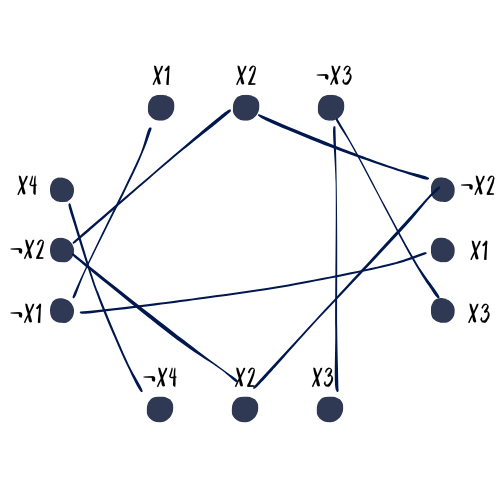
\includegraphics[width=0.45\linewidth]{figures/lec/reduction_2.png}
  \end{figure}
\end{frame}

% Slide 3
\begin{frame}
  \frametitle{Step 3}

Add all edges among vertices of the same clause \\
  (k = number of clauses)

  \begin{figure}[h!]
    \centering
    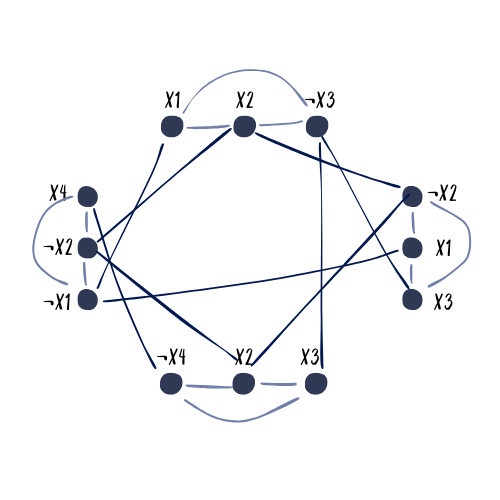
\includegraphics[width=0.45\linewidth]{figures/lec/reduction_3.png}
  \end{figure}
\end{frame}

% Slide 4
\begin{frame}
  \frametitle{Step 4}

Independent set:

  \begin{figure}[h!]
    \centering
    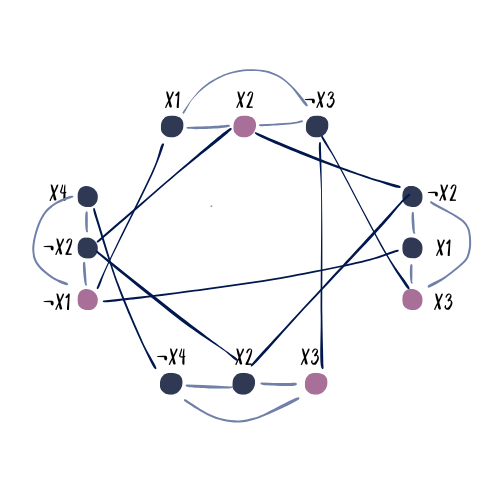
\includegraphics[width=0.45\linewidth]{figures/lec/reduction_4.png}
  \end{figure}
\end{frame}
\end{document}